\chapter{Methodology}
In this chapter, the methodologies and tools for preparing the dataset, designing the model and experiment will be introduced. 
\section{Dataset Preparation}
    \subsection{Generate dataset manually}
    The stereo vision camera, fixed on the workbench, is implemented for takes pictures of wire harness \autoref{stereoCamera1}. Once the photograph is completed, the images will be uploaded and stored 
    in the bucket to the database MinIO.
    \begin{figure}
        \centering
        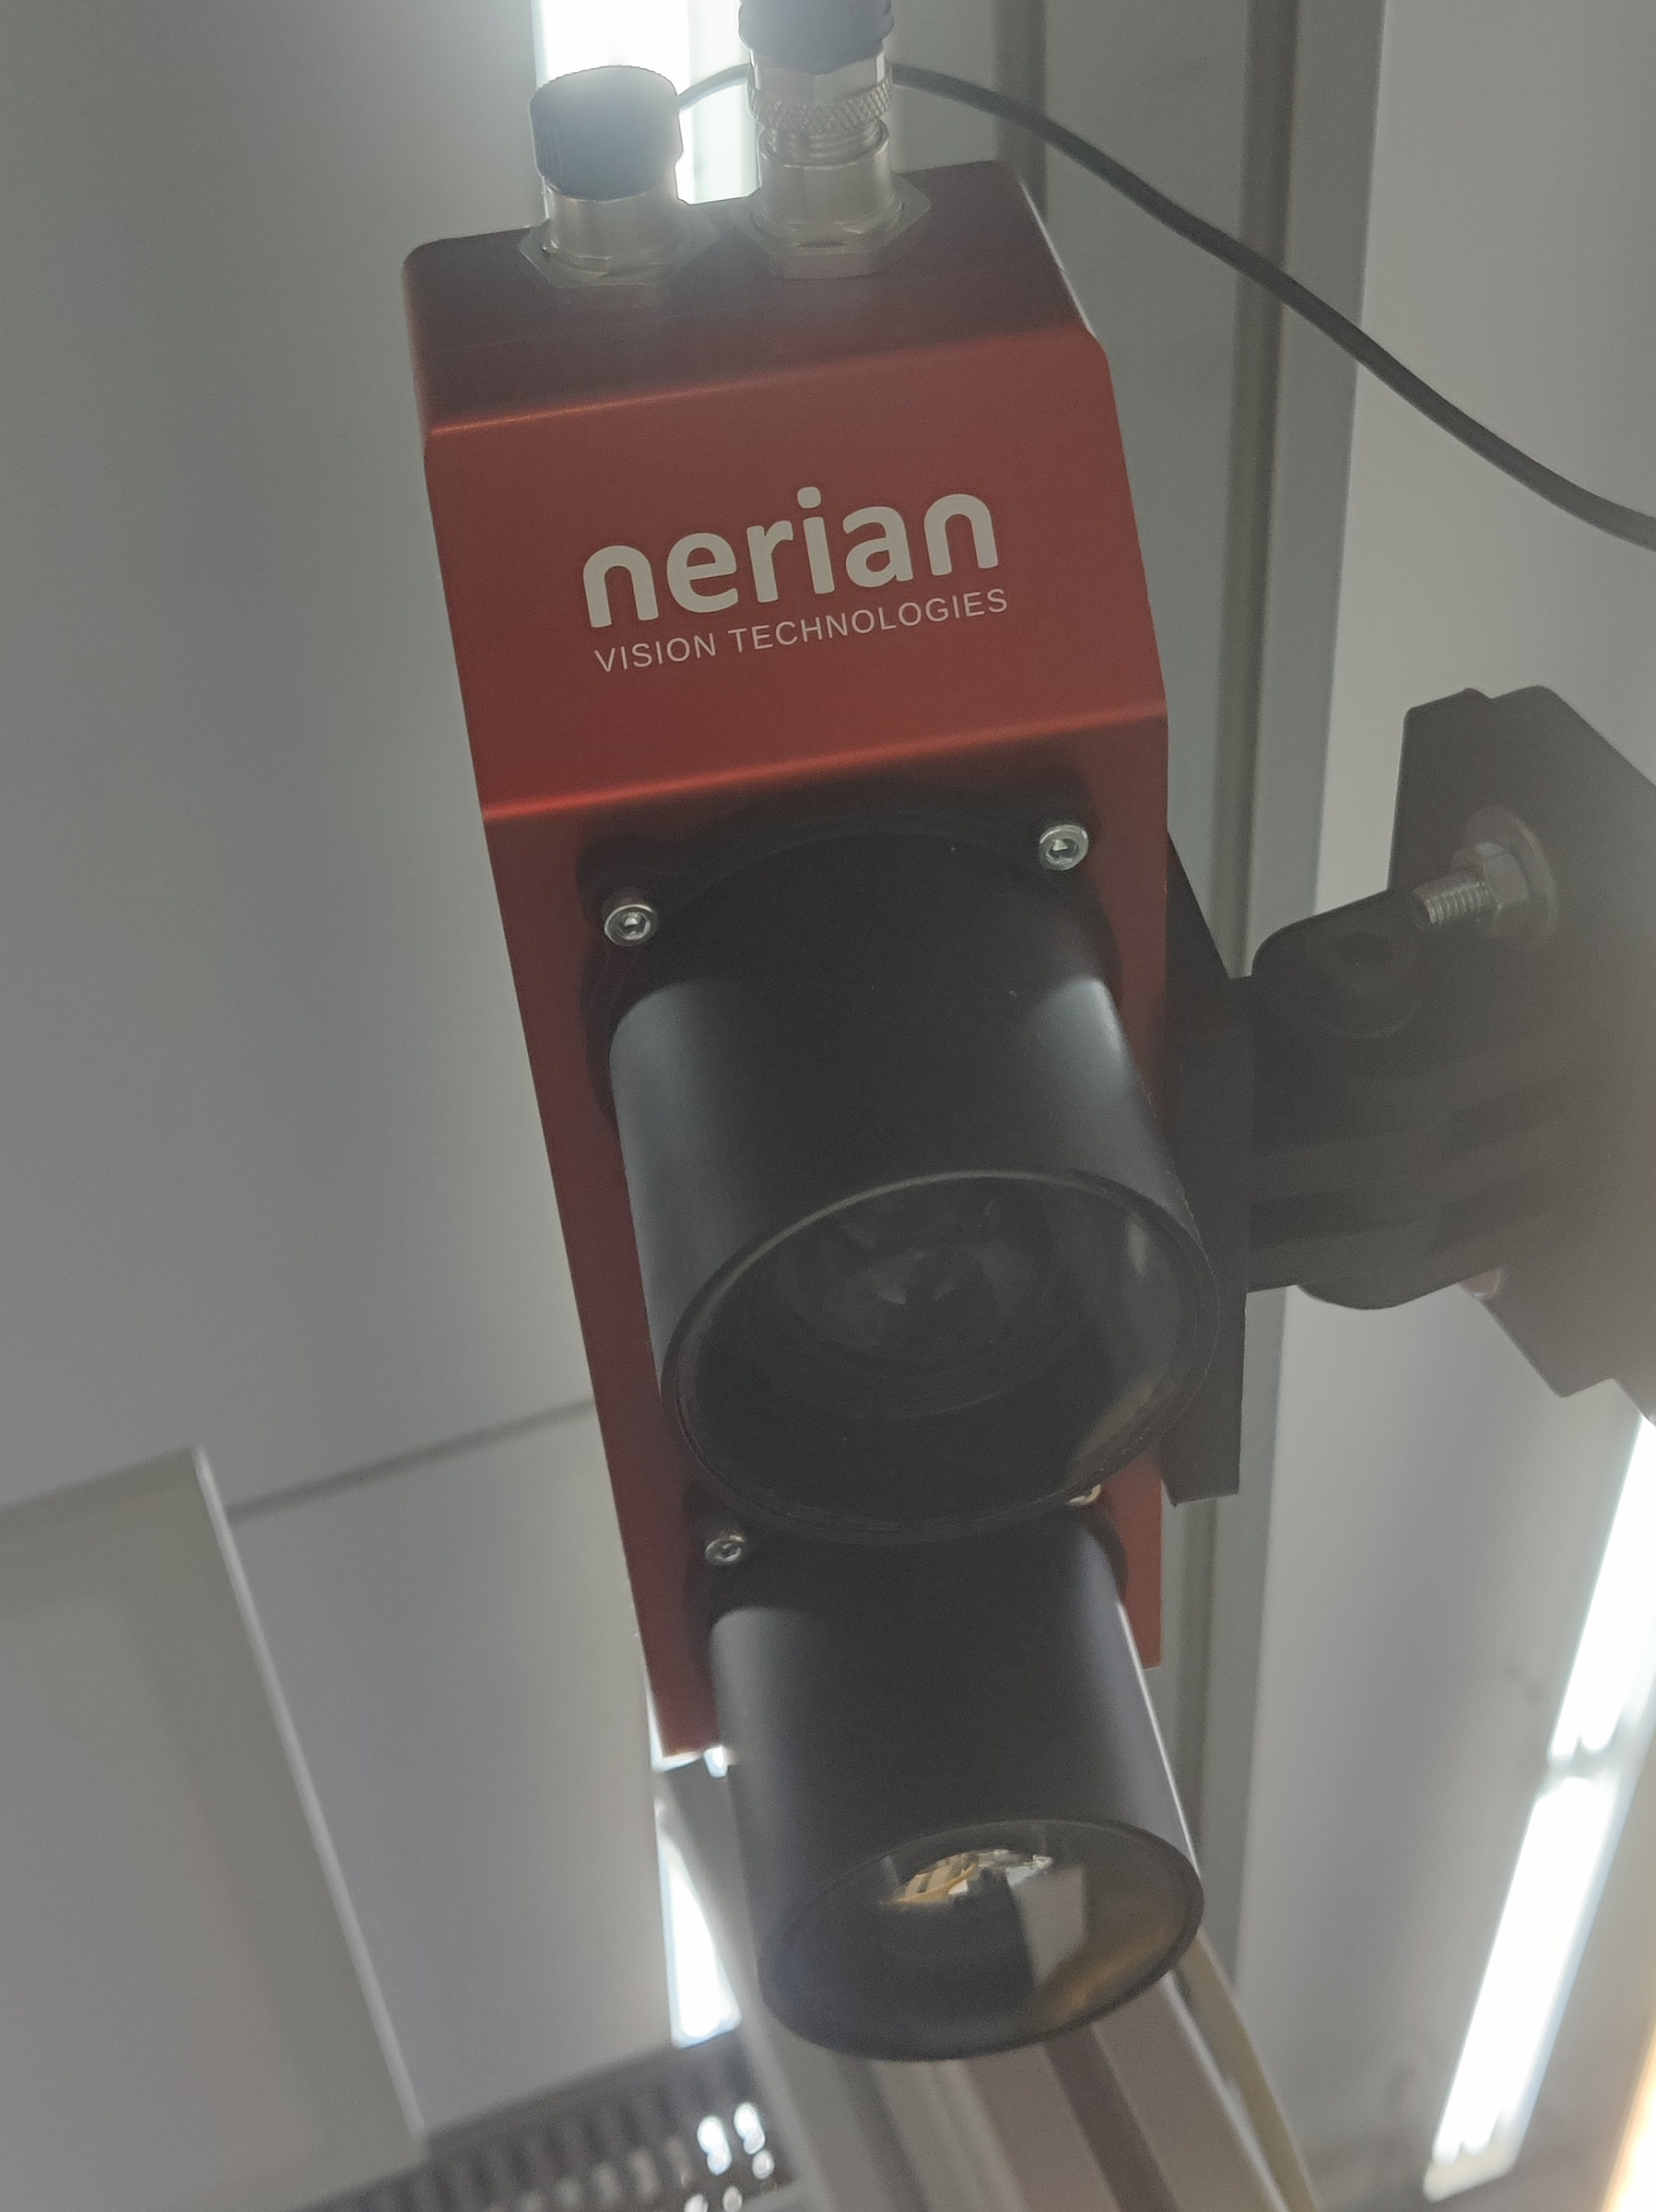
\includegraphics[width=0.4\linewidth]{example_images/stereoCamera1.jpg}
        \caption{Stereo Vision Camera}
        \label{stereoCamera1}
    \end{figure}
    Label studio\cite{LabelStudio} is a popular open-source data labeling tool. It could annotate for different vision tasks, e.g., keypoint detection, object segmentation, image classification.
    Howerver, the goal of this thesis is to construct the spline model of the wire harness by interpolating the keypoints, while the Label studio could only show the annotated keypoints in image.
    An annotation tool is developed through NiceGUI\cite{schindler2024nicegui}, which is a python-based UI framework and will show up in the web browser. The web interface of the annotation tool'
    is shown in \autoref{Annotation tool}. The user could select the bucket in dataset and load the images in this tool. Once the images are loaded, the annotation could begin.
    Click on the segment of the wire harness to create nodes. When there are more than four nodes on the segment, the cubic spline is 
    automatically interpolated. The positions of $n+1$ nodes are defined as $(x_k, y_k)$ for $k = 1, 2, ...n+1$, then the cubic spline between nodes $(x_k, y_k)$ and $(x_{k+1}, y_{k+1})$ is shown in
    \autoref{eq:cubic spline}. The neighboring splines need to fulfill the first and second order boundary conditions in \autoref{eq:boundary conditions}. 
    \begin{equation}
        \begin{aligned}
            &s_k(x) =  c_{k,3}x^3+c_{k,2}x^2+c_{k,1}x+c_{k,0}\\
            &s_k(x_k) = y_k,  s_k(x_{k+1}) = y_{k+1}
            \label{eq:cubic spline}
        \end{aligned}
    \end{equation}
    \begin{equation}
        \begin{aligned}
            s_k'(x_{k+1}) &= s_{k+1}'(x_{k+1})\\
            s_k''(x_{k+1}) &= s_{k+1}''(x_{k+1})
            \label{eq:boundary conditions}
        \end{aligned}
    \end{equation}
    The length and bending energy of the spline are calculated. The spline curve actually consists of numerous points.  The length of the entire spline curve 
    is obtained by summing the Euclidean distances of neighboring discrete points. The algorithm is shown in \autoref{Calculate the length of a spline}.
    \begin{algorithm} 
        \caption{Calculate the length of a spline}
        \label{Calculate the length of a spline}
        \begin{algorithmic}[1]
        \STATE \textbf{Input:} $X$
        \STATE $Length \leftarrow [\quad]$
        \FOR{$(x_{k},y_{k}),(x_{k+1},y_{k+1}) \in X$}
            \STATE $Distance \leftarrow \sqrt{(x_{k+1}-x_{k})^2+(y_{k+1}-y_{k})^2}$
            \STATE $Length.append(Distance)$
        \ENDFOR
        \RETURN $\text{sum}(Length)$
        \end{algorithmic}
    \end{algorithm}
    The benging energy is calcultated as \autoref{eq:bending energy}, where $\kappa(s)$ is the curvature of the spline as a function of the arc length s.
    \begin{equation}
        \begin{aligned}
            E = \int_{0}^{L} \kappa(s)^2ds
            \label{eq:bending energy}
        \end{aligned}
    \end{equation}
    The spline is defined in parametric form as $s(t) = (x(t),y(t))$ and the curvature spline be calculated as \autoref{eq:curvature}. 
    \begin{equation}
        \begin{aligned}
            \kappa(t) = \frac{\dot{x}(t) \ddot{y}(t) - \dot{y}(t) \ddot{x}(t)}{(\dot{x}(t)^2 + \dot{y}(t)^2)^{3/2}}
            \label{eq:curvature}
        \end{aligned}
    \end{equation}
    The whole equation could be represented in discrete form in \autoref{eq:curvature discrete form}.
    \begin{equation}
        \begin{aligned}
            E = \int_{0}^{L} \kappa(s)^2 \, ds = \int_{t_0}^{t_1} \kappa(t)^2 \left( \sqrt{\dot{x}(t)^2 + \dot{y}(t)^2} \right) \, dt
            \label{eq:curvature discrete form}
        \end{aligned}
    \end{equation}
    After one branch is labeled, the user could press up key to start labeling the next segment. The number of nodes on each segment should be the same. The sequences of 
    segments could also be adjusted. This is important for the model to learn the structure of the wire harness when the segments are not sorted in the program or the complexity 
    is too high to sort. Once all the segments are labeled, the annotations could be saved and exported as json file.
    \begin{figure}
        \centering
        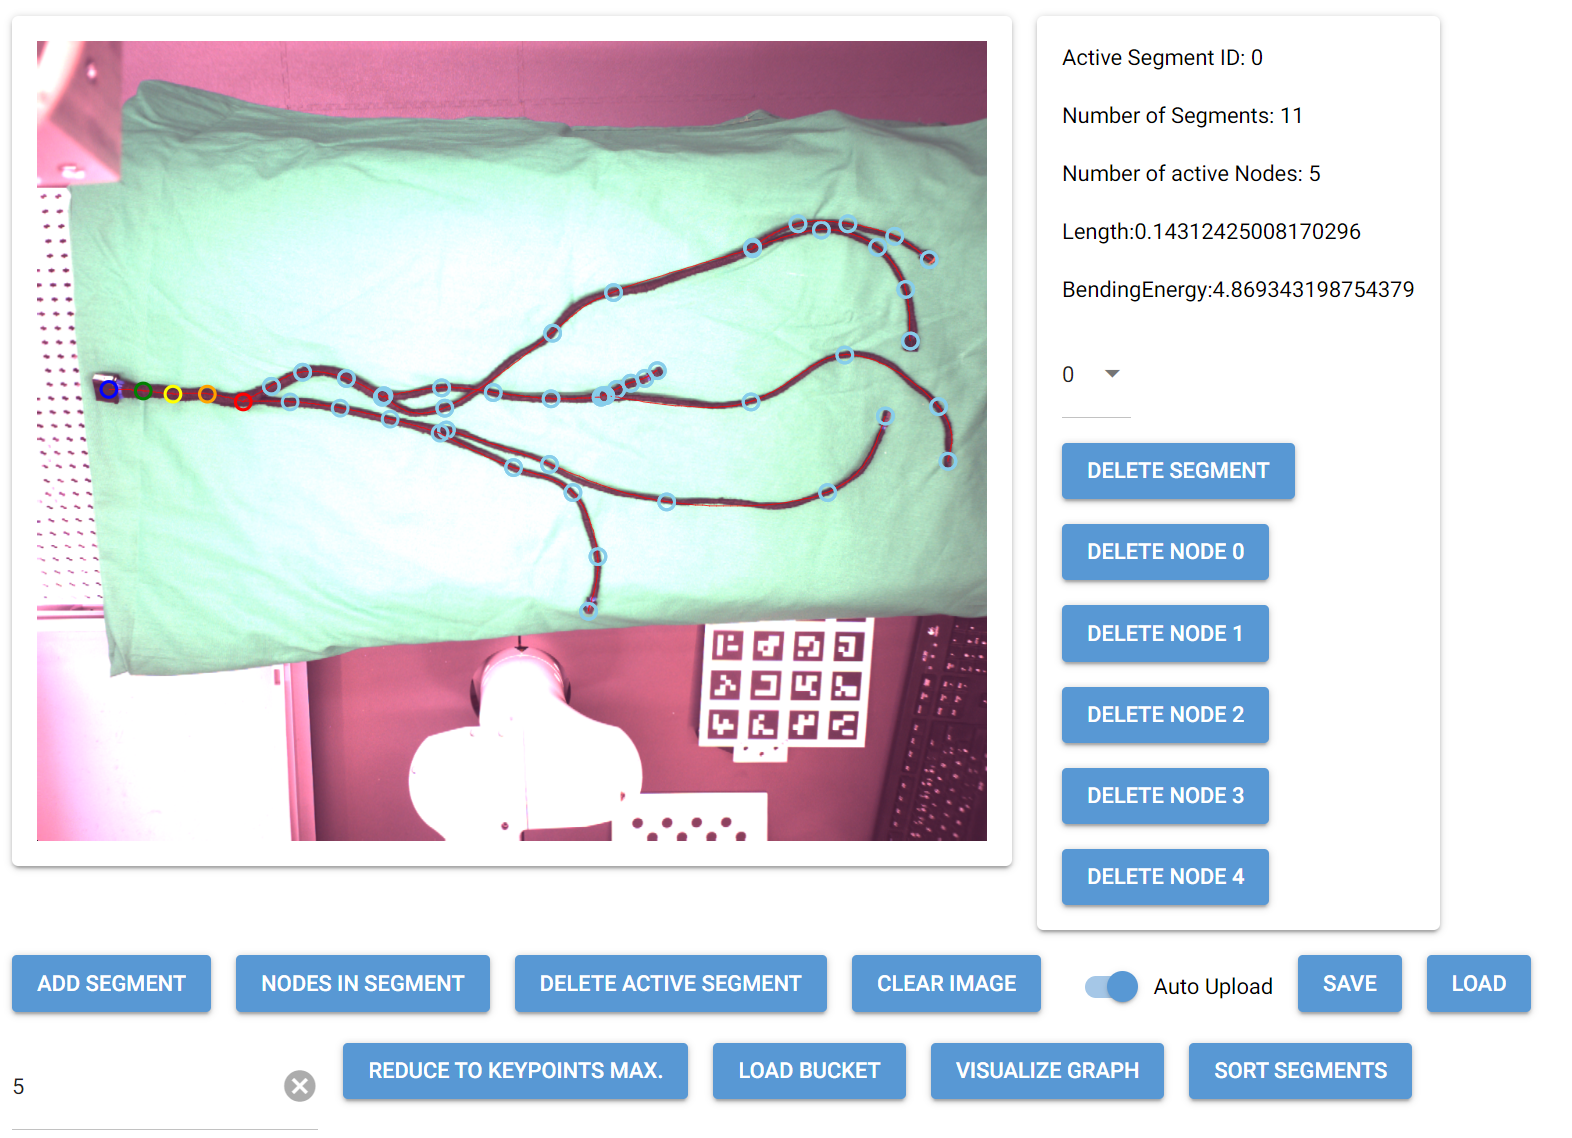
\includegraphics[width=0.9\linewidth]{example_images/NiceGUIInterface.png}
        \caption{Annotation tool}
        \label{Annotation tool}
    \end{figure}
\subsection{Dataset Expansion}
    Last subsection shows the approach of generating the dataset of the wire harness by using stereo vision camera and the annotation tool. Although this is an accurate approach
    to generate the dataset, it is time-consuming and inefficient. And the number of images labeled in this way is limited. In this subsection, two developed methods for expanding
    the datasets are introduced.
\subsubsection{Synthesized images of BDLOs}
\subsubsection{Operations on segments}
\section{Model}
\section{Experiment}